\documentclass[11pt]{article}
\usepackage[scaled=0.92]{helvet}
\usepackage{geometry}
\geometry{letterpaper,tmargin=1in,bmargin=1in,lmargin=1in,rmargin=1in}
\usepackage[parfill]{parskip} % Activate to begin paragraphs with an empty line rather than an indent %\usepackage{graphicx}
\usepackage{amsmath,amssymb, mathrsfs,  mathtools, dsfont}
\usepackage{tabularx}
\usepackage{tikz-cd}
\usepackage[font=footnotesize,labelfont=bf]{caption}
\usepackage{graphicx}
\usepackage{xcolor}
%\usepackage[linkbordercolor ={1 1 1} ]{hyperref}
%\usepackage[sf]{titlesec}
\usepackage{natbib}
%\usepackage{tikz-cd}

\usepackage{../../Tianpei_Report}

%\usepackage{appendix}
%\usepackage{algorithm}
%\usepackage{algorithmic}

%\renewcommand{\algorithmicrequire}{\textbf{Input:}}
%\renewcommand{\algorithmicensure}{\textbf{Output:}}



\begin{document}
\title{Lecture 1: Fundamental Concept of Statistical Learning}
\author{ Tianpei Xie}
\date{ Jul. 25th., 2015 }
\maketitle
\tableofcontents
\newpage
\section{Fundamental  Concepts and Assumptions}
\subsection{Categories of Machine Learning}
\begin{itemize}
\item \begin{remark} (\textbf{\emph{Categories of Machine Learning}})\\
The field of machine learning has branched into several subfields dealing with different types of learning tasks. We give a rough taxonomy of learning paradigms, aiming to provide some perspective of where the content of this book sits within the wide field of machine learning.
\end{remark}

\item \begin{remark} (\emph{\textbf{Supervised Learning}, \textbf{Unsupervised Learning} and \textbf{Reinforcement Learning}}) 
\begin{enumerate}
\item \textbf{Supervised learning}.  \underline{Learning to \emph{\textbf{predict}} and \emph{\textbf{generalize}}}. In other words, the task of learning is to infer a mapping between covariates (data) and responses (target) so that the error/cost is minimized. Each example is a description of situation (sample) together with a specification (label) of the correct action the system should take to that action. Supervised learning is an \textbf{error-correction} process. It is an one-step prediction. Human label is used as  \underline{\textbf{\emph{instructive feedbacks}}}. 

\item \textbf{Unsupervised learning}.  \underline{Learning to \emph{\textbf{represent}} and \emph{\textbf{discover}} the  \emph{\textbf{hidden structure}}} of data. A proper representation of data facilitates knowledge discovery and improves the performance of prediction. It also helps in visualization, storage and communication. 

\item \textbf{Reinforcement learning}. \underline{Learning from \emph{\textbf{interaction}}}. As compared to above approaches,  reinforcement learning studies \underline{\emph{goal-directed}} \emph{learning from interaction}. The term 'learning' means learning to map \emph{situations} to  \underline{\emph{actions}} so as to maximize the reward. Also it is often unrealistic to obtain all examples of desired behavior that are both correct and representative of all situations in which the agents have to act. Reinforcement learning is a \textbf{\emph{trial-and-error}} process and it is a multi-step prediction. It cares about future rewards in multiple steps. On the other hand, reinforcement learning only optimize the future rewards, where the rewards are used as  \underline{\textbf{\emph{evaluative feedbacks}}}.  
\end{enumerate}
\end{remark}

\item  \begin{remark} (\emph{\textbf{Active Learning}, \textbf{Passive Learning}}) \\
Learning paradigms can vary by \emph{\textbf{the role} played by the \textbf{learner}}. We distinguish between ``\emph{active}" and ``\emph{passive}"  learners. 
\begin{enumerate}
\item An \emph{\textbf{active}} learner interacts with the environment at training time, say, by posing queries or performing experiments;
\item A \emph{\textbf{passive}} learner only observes the information provided by the environment (or the teacher) without influencing or directing it.
\end{enumerate}  
\end{remark}

%\item \begin{remark} (\emph{\textbf{Online Learning}, \textbf{Batch Learning}}) \\
%The main distinct feature of \emph{\textbf{online learning}} are as follows:
%\begin{enumerate}
%\item the online learner has to \emph{\textbf{respond online}}, \emph{\textbf{throughout the learning process}}
%
%\item 
%\end{enumerate}
%
%\emph{the situations} in which , and \emph{settings} in which the learner has to \emph{\textbf{engage the acquired expertise}} only after having a chance to process large amounts of data.
%\end{remark}

\item These notes are mainly about \emph{\textbf{supervised learning} tasks}.  
\end{itemize}
\subsection{Data, Concept and Hypotheses}
\begin{itemize}
\item \begin{remark} (\emph{\textbf{Data}})\\
Define an \emph{\textbf{observation}} as a $d$-dimensional vector $x$. The \emph{unknown} nature of the observation is called a \emph{\textbf{class}}, denoted as $y$. The domain of observation is called an \emph{\textbf{input space} or \textbf{feature space}}, denoted as $\cX\subset \bR^{d}$, whereas the domain of class is called the \emph{\textbf{target space}}, denoted as $\cY$. For \emph{\textbf{classification task}}, $\cY= \set{1,\ldots, M}$; and for \emph{\textbf{regression task}}, $\cY = \bR$. 
Denote a collection of $n$ \emph{\textbf{samples}} as 
\begin{align*}
\cD \equiv \cD_n = \paren{(X_1, Y_1) \xdotx{,} (X_n, Y_n)}.
\end{align*} Note that $\cD_n$ is a finite \emph{\textbf{sub-sequence}} in $(\cX \times \cY)^n$.
\end{remark}


\item \begin{definition} (\emph{\textbf{Concept Class as a Function Class}})\\
 A \underline{\emph{\textbf{concept}}} $c: \cX \rightarrow \cY$ is the \emph{input-output association} from the nature and is \emph{to be learned} by \emph{\textbf{a learning algorithm}}.  Denote $\cC$ as \emph{the set of all concepts} we wish to learn as the \underline{\emph{\textbf{concept class}}}. That is, $\cC \subseteq \set{c: \cX \rightarrow \cY } =\cY^{\cX}.$ Concept class $\cC$ is a \emph{function class}. 
\end{definition}

\item \begin{definition} (\emph{\textbf{Hypothesis and Hypothesis Class}})\\
The learner is requested to output a \emph{prediction rule}, $h : \cX \to \cY$. This function is also called a \emph{\textbf{predictor}}, a \emph{\textbf{hypothesis}}, or a \emph{\textbf{classifier}}. The predictor can be used to predict the label of new domain points. 

Note that $\cH$ and $\cC$ may not overlap, since the concept class is unknown to learner. 
\end{definition}
\end{itemize}

\subsection{Deterministic and Stochastic Scenario}
Learning is formalized into two different \emph{scenarios}:
\begin{enumerate}
\item  \underline{\emph{\textbf{Deterministic}} \emph{Scenario}}: \\
Assume that there exist measurable space $(\cX, \srB)$, where $X \in \cX$ is the \emph{\textbf{random vector}} in $\cX$, i.e. 
\begin{align*}
X: (\Omega, \srF, \bP) \to (\cX, \srB)
\end{align*} is $\srF/\srB$ measurable. Let $\cP_{X}$ be \emph{the induced probability distribution} on $X$.

\begin{remark} (\emph{\textbf{Sample in Deterministic Scenario}})\\
\emph{In deterministic scenario}, let $X = \paren{X_1 \xdotx{,} X_n}$ be a sequence of $n$ \emph{\textbf{independent identically distributed} (i.i.d.) \textbf{random samples}}, where $X_i \sim \cP_X$. Then $Y_i = c(X_i)$ for $i=1 \xdotx{,} n$ and the sample set
\begin{align*}
\cD \equiv \cD_n = \paren{(X_1, Y_1) \xdotx{,} (X_n, Y_n)} \equiv  \paren{(X_1, c(X_1)) \xdotx{,} (X_n, c(X_n))} .
\end{align*} Note that the probability distribution for $\cD_n$ is $\cP_X^n := \otimes_{i=1}^n\cP_X$.
\end{remark}

\item  \underline{\emph{\textbf{Stochastic}} \emph{Scenario}}: \\
Assume \emph{both} $X$ and $Y$ are random, i.e. there exists a  probability space $(\cX \times, \cY, \srB, \cP_{X,Y})$ so that
\begin{align*}
(X, Y): (\Omega, \srF, \bP) \to (\cX \times \cY, \srB, \cP_{X,Y} )
\end{align*} so that the pair $(X, Y)$ is $\srF/\srB$ measurable. Let $\cP_{X, Y}$ be \emph{the induced \textbf{joint probability distribution}} on $(X, Y)$.

\begin{remark} (\emph{\textbf{Sample in Stochastic Scenario}})\\
\emph{In stochastic scenario}, the sample set 
\begin{align*}
\cD \equiv \cD_n:= \paren{(X_1, Y_1) \xdotx{,} (X_n, Y_n)}.
\end{align*} is a collection of $n$ \emph{\textbf{independent identically distributed} (i.i.d.) \textbf{random sample pairs}} $(X_i, Y_i) \sim \cP_{X, Y}$
Note that  the probability distribution for $\cD_n$ is $\cP_{X,Y}^n := \otimes_{i=1}^n\cP_{X, Y}$.
\end{remark}
\end{enumerate}

\begin{itemize}
\item \begin{remark} (\emph{\textbf{Learning Task in Deterministic Scenario}})\\
Given a collection of \emph{i.i.d.  samples} $\cD$ generated by $\cP_{X}$, a \underline{\emph{\textbf{learner}}}  considers a \emph{\textbf{fixed} subset of concepts}  $\cH\subset \cC$, which is referred as a \underline{\emph{\textbf{hypothesis class}}}, and provides a \emph{\textbf{hypothesis}} or a \underline{\emph{\textbf{classifier}}} or a \emph{\textbf{decision function}} $h \in \cH \subset \cY^{\cX}$ based on $\cD$. The task of \underline{\emph{\textbf{supervised learning}}} is to minimize \emph{\textbf{the generalization error}} given a set of training data $\cD_n$.
\end{remark}

\item \begin{remark} (\emph{\textbf{Learning Task in Stochastic Scenario}})\\
Given \emph{the sample set} $S$ generated from a \emph{(joint) probability distribution} $P_{X, Y}$. Given a fixed hypothesis class $\cH$, the task of learner is to find a hypothesis $h \in \cH$ so that the \emph{\textbf{generalization error}} or the \emph{risk} or simply the \emph{\textbf{error}} is \emph{minimized}. 
\end{remark}

\item \begin{remark} (\emph{\textbf{Deterministic} vs. \textbf{Stochastic}})\\
The main difference between these two settings is the assumption on $Y$:
\begin{enumerate}
\item \emph{\textbf{In deterministic scenario}}, $Y = c(X)$ for some \emph{\textbf{unknown} but \textbf{deterministic}} $c \in \cC$ and the learning task is to approximate $c$ by some function $h  \in \cH$.

\item \emph{\textbf{In stochastic scenario}}, $Y$ is a \emph{\textbf{random variable}}, \emph{\textbf{generated jointly} with the feature $X$} by some unknown distribution $\cP_{X, Y}$. 

The pair $(X, Y)$ \emph{may not follow} a \emph{\textbf{function relationship}}. Note for a pair $(x, y) \in \cX \times \cY$ to follow function relationship, for \emph{each given} $x$, there \emph{can only be one} correspoding $y \in \cY$. Under the stochastic assumption, \emph{any pair $(x,y)  \in \cX \times \cY$ would appear} as long as the corresponding measure $\cP_{X,Y}(x, y) >0$. 
\end{enumerate}
\end{remark}
\end{itemize}
\subsection{Generalization Error}
\begin{itemize}
\item We define \emph{\textbf{the error of a classifier}} to be the probability that it does not predict the correct label on a random data point generated by the
aforementioned underlying distribution.
\begin{definition} (\emph{\textbf{Generalization Error in Deterministic Scenario}})  \citep{mohri2018foundations}\\
Under \emph{a deterministic scenario}, \underline{\emph{\textbf{generalization error}}} or the \underline{\emph{\textbf{risk}}} or simply \underline{\emph{\textbf{error}}} for the \emph{classifier} $h \in \cH$ is defined as
\begin{align}
L(h) \equiv L_{\cP, c}(h)  &= \cP\set{h(X) \neq c(X)} \equiv \E{X}{\ind{h(X)\neq c(X)}}\label{expr: gen_err_determin}
\end{align}
with respect to the concept $c \in \cC$ and \emph{the feature distribution} $\cP \equiv \cP_X$.
\end{definition}

\item Similarly, under the stochastic scenario, the joint distribution $\cP_{X, Y}$ has replaced the concept class $c$:
\begin{definition} (\emph{\textbf{Generalization Error in Stochastic Scenario}})  \citep{mohri2018foundations}\\
In \emph{stochastic scenario}, \underline{\emph{\textbf{generalization error}}} or the \emph{\textbf{risk}} or simply \emph{\textbf{error}} for the \emph{classifier} $h \in \cH$ is defined as
\begin{align}
L(h) \equiv  L_{\cP}(h) &= \cP\set{h(X) \neq Y}\equiv \E{X, Y}{\ind{h(X)\neq Y}} \label{expr: gen_err_gener}
\end{align} with respect to the joint distribution $\cP \equiv \cP_{X, Y}$.
\end{definition}

\item \begin{remark}
Under both situations, \emph{the generalization error} $L(h)$ is a \emph{\textbf{functional}} on both the \emph{\textbf{hypothesis}} $g$ and \emph{the underlying \textbf{data generating process}}, defined by distribution $\cP$.
\end{remark}
\end{itemize}

\subsection{Empirical Risk Minimization}
\begin{itemize}
\item \begin{remark} (\textbf{\emph{Assumption}})\\
The learner is blind to the underlying distribution $\cP$ over the world and to the labeling concept $c$. 
\end{remark}

\item  Since the learner does not know what $\cP$ and $c$ are, \emph{the generalization error} is not directly available to the learner. A useful notion of error that can be calculated by the learner is \emph{the training error} or \emph{empirical error}: 
\begin{definition} (\emph{\textbf{Empirical Error or Training Error}}) \\
Given the data $\cD_n$, the \emph{\textbf{training error}} or \underline{the \emph{\textbf{empirical error/risk}}} of a hypothesis $h \in \cH$ is defined as 
\begin{align*}
\widehat{L}(h)   \equiv \widehat{L}_{\cD_n}(h)  &= \frac{1}{n}\sum_{i=1}^{n}\ind{h(X_i)\neq Y_i} = \frac{1}{n}\abs{\set{i: h(X_i)\neq Y_i}} := \Em{}{\ind{h(X) \neq Y}}
\end{align*} where either $Y = c(X)$ or $Y$ is a random variable associated with $X$.
\end{definition}

\item \begin{definition} (\textbf{\emph{Empirical Risk Minimization (ERM)}}) \\
\underline{\emph{\textbf{The Empirical Risk Minimization (ERM)}}} is a learning paradigm that aims at finding the optimal classifer $h \in \cH$ by \emph{\textbf{minimizing the empirical error}} $\widehat{L}_{\cD}(h)$; i.e.
\begin{align*}
h^{*} \equiv h^{*}_{\cD} \in \arg\min_{h \in \cH}\widehat{L}_{\cD}(h)
\end{align*}
\end{definition}

\item \begin{remark} (\textbf{\emph{Empirical Risk Minimization with Inductive Bias}}) \\
The hypothesis class $\cH$ is usually chosen as a subset of concept class $\cC$. Thus \emph{the empirical risk minimization (ERM)} may lead to a \emph{biased} predictor $h \in \cH$ that is not optimal in $\cC$. Such restrictions are often called \underline{\emph{\textbf{an inductive bias}}}.  Since \emph{the choice of such a restriction $\cH$} is determined \emph{\textbf{before}} the learner \emph{sees the training data}, it should ideally be based on some \emph{\textbf{prior knowledge}} about the problem to be learned. 
\end{remark}

%\item \begin{remark}
%Not to be confused with $L_n(g) := L(g_n) = \cP_{X,Y}\set{g_n(X)\neq Y}$, where the subscript $n$ indicates  the dependency of $g$ on $\cD_n$.
%\end{remark}
\end{itemize}

\subsection{Bayes Error}
\begin{itemize}
\item  \begin{definition} (\emph{\textbf{Bayes Error}})\\
Under a given distribution $\cP$,  the \underline{\emph{\textbf{Bayes error}}} or \underline{\emph{\textbf{Bayes risk}}} is defined as 
\begin{align}
L^{*} \equiv L_{\cP}^{*} &= \inf_{h}\set{L_{\cP}(h)}, \label{expr: Bayes_err}
\end{align} where the infimum is with respect to \emph{all measureable function} $h: \cX \rightarrow \cY$. And the \emph{hypothesis} $h^{*}$ such that $L_{\cP}(h^{*})= L^{*}$ is called the \underline{\emph{\textbf{Bayes classifier}}}.
\end{definition}

\item \begin{remark} (\textbf{\emph{Bayes Error as Functional of Distribution}})\\
\emph{\textbf{Bayes Error} is \textbf{a functional of underlying distribution $\cP$ only}} and it does not depend on choice of function $h$ or function class $\cH$.
\begin{align*}
 L^{*} \equiv L_{\cP}^{*} &=  L^{*}(\cP).
\end{align*} Intuitively, it reflects \emph{how hard the learning problem} is \emph{\textbf{intrinsically}} since it determines \emph{\textbf{the lower bound} of generalization error}.
\end{remark}

\item \begin{remark}  (\emph{\textbf{Bayes Error in Deterministic Scenario}})\\
Under \emph{\textbf{the deterministic}} setting, the Bayes error is $L^{*}=0$ since by assumption $Y = c(X)$ for some $c \in \cC$, thus the infimum is zero. 
\end{remark}

\item \begin{remark} (\emph{\textbf{Bayes Classifier if $\cP_{X, Y}$ is Known}})\\
The learning task is concerning about the situation when $\cP_{X, Y}$ is \emph{\textbf{unknown}} but \emph{\textbf{if $\cP_{X, Y}$ is \underline{known}}}, then \emph{\textbf{the optimal hypothesis}} is known as \emph{\textbf{the posterior conditional expectation}}:
\begin{align*}
\eta(X) := \cP[Y | X] &= \frac{d \cP_{X, Y}}{d \cP_{X}}
\end{align*} Note that $\cP[Y | X]_{\omega}$ is a function of $X$ given each $\omega \in \Omega$, which means that $g(X, \omega) := \cP[Y | X]_{\omega}$ is a random function itself.
For $\cY = \set{0,1}$ and $X$ be discrete random variables, it can be written as 
\begin{align}
\eta(x) &= \cP\set{Y=1 \big| X=x} \nonumber\\
 &= \E{p(y|x)}{y\big|\,X=x}. \label{expr: cond_Prob_fun}
\end{align} 
and \emph{\textbf{the Bayes classifier}} (decision function)
\begin{align}
h^{*}(x)  &= \argmax\limits_{y\in \set{0,1}}P(Y| X=x)\nonumber\\
&=\left\{ \begin{array}{cc}
1 & \eta(x) > \frac{1}{2} \\ 
0 & \text{o.w.}
\end{array} \right. \label{expr: Bayes_classif}
\end{align} with the corresponding \emph{\textbf{Bayes error}}
\begin{align}
L^{*}&=\E{P(X)}{\min\set{ P(Y=y| X) \;|\; y\in \set{0, 1 }}} \nonumber\\
&= 1- \E{P(X)}{ \eta(X)\ind{\eta(X)>1/2} + (1-\eta(X))\ind{\eta(X)\le 1/2}  }
\end{align}
\end{remark}

\item We summarizes our discussion as follows
 \begin{proposition} (\textbf{Conditional Estimator is Bayes Classifer if Distribution is Known}) \citep{devroye2013probabilistic}\\
Given the posterior (conditional) probability $\eta(x)= \cP(Y=1|X=x)= \E{p(y|x)}{Y| X=x}$, where $\cP(X,Y)$ is the underlying distribution of data and the Bayes decision function  
\begin{align*}
h^{*}(x) &= \ind{\cP(Y=1| X=x)>1/2}\\
&=  \ind{\E{p(y|x)}{y\big|\,X=x}>1/2},
\end{align*}
for any decision function $g: \cX \rightarrow \set{0,1}$, 
\begin{align*}
\cP\set{h^{*}(X)\neq Y} &\le \cP\set{h(X) \neq Y}
\end{align*}
\end{proposition}
\begin{proof}
Given $X=x$, the conditional error probability of any $g$ can be expressed as
\begin{align}
&\cP\set{h(X) \neq Y| X=x}  \nonumber\\
&= 1- \cP\set{ Y= h(X)| X=x }\nonumber\\
&=1- \paren{\cP\set{Y=1, h(X)=1 | X=x}+ \cP\set{Y=0, h(X)=0 | X=x}}\nonumber\\
&=1- \paren{ \ind{h(X)=1}\cP\set{ Y=1 | X=x } + \ind{h(X)=0}\cP\set{ Y=0 | X=x }    } \nonumber\\
&=1- \brac{ \ind{h(X)=1} \eta(x) +  \ind{h(X)=0}\paren{1- \eta(x)}}  \label{expr: Bayes_error_expr}
\end{align}
For any $x\in \cX$, 
\begin{align*}
&\cP\set{h(X)\neq Y| X=x} - \cP\set{h^{*}(X)\neq Y| X=x}\\
&= \eta(x)\paren{  \ind{h^{*}(x)=1} -  \ind{h(x)=1}  }+ (1-\eta(x))\paren{\ind{h^{*}(x)=0} -  \ind{h(x)=0}}\\
&= (2\eta(x)-1)\paren{ \ind{h^{*}(x)=1} -  \ind{h(x)=1}  }\\
&\ge 0,
\end{align*}
since $h^{*}(x)=1$ if and only if $(2\eta(x)-1)>0$ and $\paren{ \ind{h^{*}(x)=1} -  \ind{h(X)=1}  }\ge 0$ if and only if $h^{*}(x)=1$. \qed
\end{proof}

\item \begin{proposition} \label{prop: plug_in_deviation} (\textbf{Plug-In Estimator}) \citep{devroye2013probabilistic}\\
Consider a plug-in decision function 
\begin{align*}
h(x) &= \ind{\tilde{\eta}(x)>1/2},
\end{align*}
where $\tilde{\eta}(x)$ is an estimate of $\eta(x)= \cP(Y=1| X=x)$, then for the error probability of plug-in decision function  $h(X)$, we have
\begin{align}
\cP\set{h(X)\neq Y} - L^{*} &= 2\int_{\cX}\abs{\eta(x)- 1/2}\ind{h(X)\neq h^{*}(x)}\mu(dx) \label{expr: Bayes_excess_plug_in}
\end{align}
and 
\begin{align}
\cP\set{h(X)\neq Y} - L^{*} &\le 2\int_{\cX}\abs{\eta(x)- \tilde{\eta}(x)}\mu(dx) \nonumber\\
& = 2\E{p(X)}{\eta(X)- \tilde{\eta}(X)}  \label{expr: Bayes_excess_plug_in_2}
\end{align}
\end{proposition}
\begin{proof}
If for some $x\in \cX$, $h(X)= h^{*}(x)$, the clearly the difference btw the conditional error probability of $g$ and $h^{*}$ is zero; i.e. 
\begin{align*}
\cP\set{h(X)\neq Y| X=x} - \cP\set{h^{*}(X)\neq Y| X=x}  &= 0.
\end{align*}
Otherwise, $h(X)\neq h^{*}(x)$, then 
\begin{align*}
&\cP\set{h(X)\neq Y| X=x} - \cP\set{h^{*}(X)\neq Y| X=x}  \\
&= (2\eta(x)-1)\paren{ \ind{h^{*}(x)=1} -  \ind{h(x)=1}  }\\
&= \abs{2\eta(x)-1}\ind{h(x)\neq h^{*}(x)}
\end{align*}
Thus
\begin{align*}
\cP\set{h(X)\neq Y} - L^{*} &=2 \int_{\cX}\abs{\eta(x)-1/2}\ind{h(x)\neq h^{*}(x)}\mu(dx)\\
&\le 2 \int_{\cX}\abs{\eta(x)- \tilde{\eta}(x)}\mu(dx),
\end{align*}
since $h(X)\neq h^{*}(x)$ implies $\abs{\eta(x)- \tilde{\eta}(x)}\ge \abs{\eta(x)-1/2}$.\qed 
\end{proof}

\item  \begin{corollary}
Consider a plug-in decision function 
\begin{align*}
h(X) &= \ind{\tilde{\eta}_{1}(x)>\tilde{\eta}_{0}(x)},
\end{align*}
where $\tilde{\eta}_{1}(x)$ is an estimate of $\eta(x)$ and $\tilde{\eta}_{0}(x)$ is an estimate of $1-\eta(x)$, then for the error probability of plug-in decision function  $h(X)$, we have
\begin{align}
\cP\set{h(X)\neq Y} - L^{*} &\le \int_{\cX}\abs{(1- \eta(x))- \tilde{\eta}_{0}(x)}\mu(dx)+ \int_{\cX}\abs{\eta(x)- \tilde{\eta}_{1}(x)}\mu(dx)
\end{align}
In particular, if $\tilde{\eta}_{1}(x) \equiv \tilde{q}_{1}\tilde{p}_{1}(x)$ and $\tilde{\eta}_{0}(x)\equiv \tilde{q}_{0}\tilde{p}_{0}(x)$, where $\tilde{q}_{1}, \tilde{q}_{0}$ are estimate of prior distribution for $\cP\set{Y=1}=q$ and $\cP\set{Y=0}=1-q$ and $\tilde{p}_{1}(x), \tilde{p}_{0}(x)$ are estimate of class conditional distribution of $x$ given $Y=1$ and $Y=0$ respectively, then 
\begin{align*}
\cP\set{h(X)\neq Y} - L^{*} &\le \int_{\cX}\abs{(1- q)p_{0}(x)- \tilde{q}_{0}\tilde{p}_{0}(x)}dx+ \int_{\cX}\abs{qp_{1}(x)- \tilde{q}_{1}\tilde{p}_{1}(x)}dx
\end{align*}
\end{corollary}



\item \begin{exercise} (\textbf{Transformation Increases Bayes Error}) \citep{devroye2013probabilistic}\\
Let $T: \cX\rightarrow \cX' $ be an arbitrary measureable function. If $L_{\cX}^{*}$ and $L_{T(\cX)}^{*}$ denote the Bayes error probability for $(X,Y)$ and $(T(X), Y)$, respectively, then prove that 
\begin{align*}
L_{T(\cX)}^{*} &\ge L_{\cX}^{*}.
\end{align*}
This shows that transformation destroys information, because the Bayes risk increases. 
\end{exercise}
\begin{proof}
We see that for any measureable set $B\subset \cX'$,  $\cP(T(X)\in B) = \cP\set{X\in T^{-1}(B)}$. Define the posterior distribution 
\begin{align*}
\eta_{T}(t) &\equiv \cP\set{Y=1| T(x)= t}\\
\eta_{T}(T(x)) &= \E{}{\eta(X)| T(x)}.\\
%\tilde{g}(T(x))&= \ind{\eta(T(x))>1/2}\\
%\Rightarrow  \eta(T(x)) \equiv \tilde{\eta}_{T}(x)&= \frac{\cP\set{Y=1, x\in T^{-1}(t)}}{\cP\set{x\in T^{-1}(t)}}\\
%\tilde{g}(T(x)) \equiv \tilde{g}_{T}(x)&= \ind{\tilde{\eta}_{T}(x) \ge 1/2} 
\end{align*} 
Use the \emph{F-error} theorem by observing that $L^{*} = d_{F}(X,Y)$ with $F(x) = \min\set{x, 1-x}$, thus
\begin{align*}
L_{T(\cX)}^{*}&=  d_{F}(T(X),Y)\\
&= \int \min\set{1- \eta_{T}(T(x)),  \eta_{T}(T(x))}p(x)\mu(dx)\\
&=  \int \min\set{1- \E{}{\eta(X)| T(x)},  \E{}{\eta(X)| T(x)}}p(x)\mu(dx)\\
&\ge \int \E{}{ \min\set{1- \eta(X), \eta(X)}  | T(x)} p(x)\mu(dx)\\
&= \int \min\set{1- \eta(x), \eta(x)}p(x)\mu(dx)\\
& = d_{F}(X,Y)=  L_{\cX}^{*}.\qed \\
\end{align*} 
\end{proof}

\begin{remark}
Note that for any measureable $T: (\cX, \cB) \rightarrow (\cX', \cB')$, let $X'= T(X)$ for $X: \Omega \rightarrow \cX$,
\begin{align*}
\E{}{Y| T(X)} &= \E{}{Y| T^{-1}(\sigma(X'))}\\
&= \E{}{Y| \rlat{\sigma(X)}{T^{-1}(\sigma(X')}}\\
& \equiv \E{}{\E{}{Y|\sigma(X)}\,|\,T(X)} \\
\text{for } E\in T^{-1}(\sigma(X'))= \sigma(T^{-1}X') &\subset \sigma(X) \subset \sigma(X,Y) \\
 \int_{E} \E{}{\E{}{Y|\sigma(X)}\,|\sigma(T^{-1}X')}dP_{X,Y}& = \int_{E} \E{}{Y|\sigma(X)} dP_{X,Y}  \\
 &= \int_{E}Y dP_{X,Y}\\
 &= \int_{E} \E{}{Y| T(X)} dP_{X,Y} \qed
\end{align*} 
\end{remark}

\item \begin{exercise}\citep{devroye2013probabilistic}\\
Let $X'$ be independent with $(X,Y)$. Show that 
\begin{align*}
L_{X', X}^{*} &= L_{X}^{*}.
\end{align*}
\end{exercise}
\begin{proof}
Just need to see that $\eta'(x',x) = \cP(Y| (X', X)= (x' , x)) = \cP(Y| X=x)= \eta(x)$ by independence, the result then follows directly. \qed
\end{proof}
\end{itemize}
\subsection{Approximation Error and Estimation Error}
\begin{itemize}
\item \begin{remark} (\emph{\textbf{Optimal Rule within Hypothesis Class}})\\
Given a hypothesis class $\cH$, the \emph{\textbf{best possible generalization error}} is obtained by
\begin{align*}
L \equiv L_{\cP, \cH} &= \inf_{h \in \cH}L_{\cP}(h)  = \inf_{h \in \cH}\cP\set{h(X) \neq Y}
\end{align*} \textbf{\emph{The optimal rule within}} $\cH$ is defined as $h_{\cH}^{*} \in \arg \inf_{h \in \cH}L_{\cP}(h) $. Note that $L \ge L^{*}$. \emph{The optimal error rate} $L_{\cP, \cH}$ is a function of $\cP$ and $\cH$.
\end{remark}

\item \begin{remark} (\emph{\textbf{Optimal Rule under Empirical Error Probability}})\\
Given a hypothesis class $\cH$, the \emph{\textbf{empirically optimal rule}} $h_{\cD}^{*}$ is given by 
\begin{align*}
h_{\cD}^{*}  \in \arg\min_{h \in \cH}\widehat{L}_{\cD}(h).
\end{align*} Since the function $h_{\cD}^{*}$ is determined by data $\cD$, it can be seen as a \emph{\textbf{random function}}
\begin{align*}
h_{\cD}^{*}(x) := h(x | \cD) \equiv  h(x | ((X_1, Y_1) \xdotx{,} (X_n, Y_n)) ).
\end{align*} In general, we use the notation $h_{\cD}$ for a hypothesis returned by a learning algorithm given data $\cD$.
\end{remark}

\begin{figure}
\begin{minipage}[t]{1\linewidth}
  \centering
  \centerline{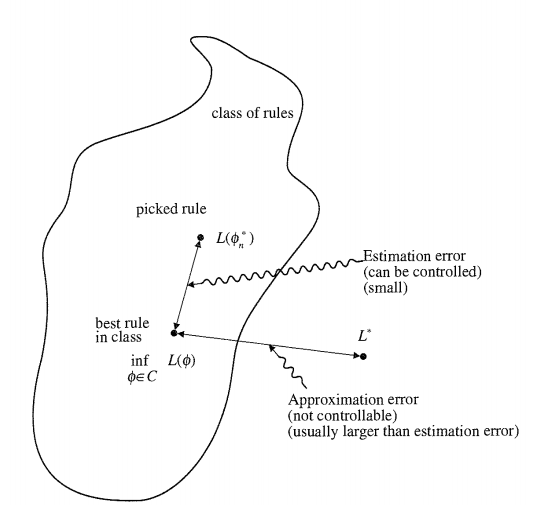
\includegraphics[scale = 0.5]{est_app_error.png}}
\end{minipage}
\caption{\footnotesize{\textbf{Estimation Error vs. Approximation Error \citep{devroye2013probabilistic}}}}
\label{fig: est_app_error}
\end{figure}

\item \begin{remark} (\emph{\textbf{Estimation Error} vs. \textbf{Approximation Error}})\\
The difference between \emph{\textbf{the optimal generalization error}} \emph{within a hypothesis class} $\cH$ and \emph{\textbf{the generalization error}} for the \emph{optimal rule} under ERM  is called \underline{\emph{\textbf{the excess risk}}}.  It is the quantity that primarily interests us:
\begin{align*}
L(h_{\cD}^{*}) - L &:= L(g_n^{*}) - \inf_{h \in \cH}L(h)
\end{align*} Note that \emph{both} quantites are \emph{\textbf{generalization error not training error}}. To compare with \emph{Bayes error}, we have the following decomposition
\begin{align*}
L(h_{\cD}^{*}) - L^{*} &= \paren{L(h_{\cD}^{*}) - \inf_{h \in \cH}L(h)} + \paren{\inf_{h \in \cH}L(h) - L^{*}}.
\end{align*} 
\begin{enumerate}
\item The first difference term is called \underline{\emph{\textbf{the estimation error}}};

\item the second difference term is called \underline{\emph{\textbf{the approximation error}}}. This latter term may be bounded in a \emph{\textbf{distribution-free manner}}, and \emph{a rate of convergence results that \textbf{only depends on the structure of $\cH$}}.
\end{enumerate}

When the sub-class of functions $\cH$ is \emph{\textbf{large}}, $L = \inf_{h \in \cH}L(h)$ may be close to $L^{*}$, but the former error, \emph{the estimation error}, is probably \emph{large} as well.  If $\cH$ is \emph{\textbf{too small}}, there is no hope to make the approximation error small.

 In empirical risk minimization, the subclass $\cH$ is \emph{\textbf{fixed}}, and we have to live with the functions in $\cH$. \emph{The best we may then
hope for is to minimize $L(h_{\cD}^{*}) - \inf_{h \in \cH}L(h)$}. 
\end{remark}

\item \begin{remark} (\emph{\textbf{Overfitting}})\\
If $\cH = \cY^{\cX}$ is the class of all (measurable) decision functions, then we can always find a classifier in $\cH$ with \emph{\textbf{zero empirical error}}, but it may have \emph{\textbf{arbitrary values} outside of the points} $X_1 \xdotx{,} X_n$. For example, an \emph{empirically optimal classifier} is
\begin{align*}
h_{\cD}^{*}(x) &= \left\{ \begin{array}{cc}
Y_i & x = X_1 \xdotx{,} X_n\\
0 & \text{otherwise}
\end{array}
\right.
\end{align*} This is clearly not what we are looking for. This phenomenon is called \emph{\textbf{overfitting}}, as the overly large class $\cH$ \emph{overfits} the data. 
\end{remark}

\item \begin{remark}: (\emph{\textbf{Statistical Decision}}) \citep{berger2013statistical}\\
The \emph{statistical learning theory} is closely related to the \emph{statistical decision theory} in which the terms such as  \emph{(Empirical) Risk/Utility}, \emph{decision function} are used as an alternative to the terms like \emph{(Empirical) Error}, \emph{hypothesis/classifier}. 
\end{remark}
\end{itemize}






%\item \begin{definition} (\emph{\textbf{Generalization Error of Estimated Hypothesis}})  \citep{devroye2013probabilistic} \\
%Given the data $\cD_n$, we can define \emph{\textbf{the conditional probability of error}}:
%\begin{align}
%L_n(g) &= L(g_n) := \cP_{X, Y}\set{g_n(X; \cD_n) \neq Y | \cD_n}\equiv \E{X, Y}{\ind{g_n(X)\neq Y} | \cD_{n}} \label{expr: gen_err_estimator}
%\end{align}  This is a random variable because it depends upon the data $\cD_n$. So, $L_n$ averages over the distribution of $(X, Y)$, but \emph{the \textbf{data} is held \textbf{fixed}}. Averaging over the data as well would be unnatural, because in a given application, one has to live with the data at hand.  %Conditioning on $g_n$, this is  \emph{the generalization error of $g_n$}. Note the term ``\emph{conditional}" is with respect to $g_n$ which is a function of sample $\cD_n$ not with respect to current input-output pair $(X,Y)$.
%\end{definition}
%

%
%



%
%\item \begin{remark}
% Note that, with abuse of notation, the subscript $n$ indicate the dependency of $g$ on $\cD_n$ not the dependency of error estimator $\widehat{L}$  on $n$. For training error estimator, both $g_n$ and $\widehat{L}$ is a function on $\cD_n$ but in general, it could be different.
% \end{remark}
%\item \begin{remark}
%Both the \emph{generalization error} and \emph{empirical error} are \emph{\textbf{functionals}} of $g \in \cH$.
%\end{remark}

%\item \begin{remark} (\emph{\textbf{Training Error} vs. \textbf{Validation Error}})\\
%Assume $\cD_n : =\set{(X_{i}, Y_{i})}_{i \in T_t}$ is the set of $\abs{T} = n$ training data, and $\cV_m : =\set{(X_{j}, Y_{j})}_{j \in T_v}$ is the set of $\abs{T_v} = m$ validation data, and $T_t \cap T_v =\emptyset$ so that $\sigma(\cD_n) \indep \sigma(\cV_m)$. 
%
%We see that 
%\begin{align*}
%\widehat{L}_{\cV_m}(g_n) = \widehat{\cP}_{m}g_n  &= \widehat{\cP}_{X, Y}\paren{\set{g(X| \cD_n)\neq Y} |  \cV_m} &&\text{ validation error}\\
%\widehat{L}_{\cD_n}(g_n) = \widehat{\cP}_{n}g_n &= \widehat{\cP}_{X, Y}\paren{\set{g(X| \cD_n)\neq Y} |  \cD_n} &&\text{ training error}\\
%L(g_n) = \cP g_n  &=\cP_{X, Y}\paren{\set{g(X| \cD_n)\neq Y}} &&\text{ generalization error}
%\end{align*}
%\end{remark}





%\item 
%\begin{definition} (\emph{\textbf{Generalization Error for Estimated Hypothesis}}) \citep{devroye2013probabilistic}\\
%(In stochastic setting,) denote $g_n$ as \emph{the estimated hypothesis} based on samples $\cD_{n} = ((X_{i}, Y_{i}), 1\le i\le n)$.
%\begin{align*}
%%g_n(\cdot) &= g(\cdot | \sigma(X_i, i \le n)) && \text{ deterministic}\\
%%\text{ or }
%g_n(\cdot) &= g(\cdot | \sigma((X_i, Y_i), i \le n)) && \text{ stochastic}
%\end{align*}
%The performance of (stochastic) classifier $g_{n}$ is measured by the \emph{\textbf{conditional probability of error}}, or the generalization error of $g_n$:
%\begin{align*}
%L_{n} = L(g_{n}) &= \cP_{X, Y}\set{g_{n}(X)\neq Y| \sigma((X_i, Y_i), i \le n)}
%\end{align*} Note 
%\begin{enumerate}
%\item For fixed $ \sigma((X_i, Y_i), i \le n)$, $g_n$ is a \emph{deterministic function}, and $L_n$ is a \emph{\textbf{functional}} of $g_n$ 
%
%\item $L_n$ itself is \emph{\textbf{a function of validation samples}} $\sigma((X_i, Y_i), i \le n)$
%\end{enumerate}
%\end{definition}
%
%\item \textbf{Remark}: One should distinguish $L(g)$, $L_{n}\equiv  L(g_{n})$ with $\widehat{L}_{n}(g)$ and $L^{*}=\inf_{g}\set{L(g)}$. 
%\begin{itemize}
%\item The first two $L(g)$, $L_{n}\equiv  L(g_{n})$ are expectation (functional) with respect to the \emph{true underlying distribution} $\cP(\cX \times \cY)$; From the first one to the second one, one  just replaces a general classifier $g\in \cH$ with a classifier (functional) $g_{n}$ trained on an independent (training) set $\cD$.
%
%\item $\widehat{L}_{n}(g)$ is (functional) of general classifier $g$ with respect to the \emph{empirical distribution} $\widehat{\cP}_{X, Y}$.
%
%\item  The Bayes error $L^{*}$ is a \emph{constant} that is only depend on the (fixed) true underlying distribution $\cP_{X, Y}$. 
%
%\item The first one is the \emph{generalization error functional}; the second one the \emph{generalization error} for \emph{\textbf{given estimated hypothesis}}, which is the \emph{\textbf{test error}}; the third one the \emph{\textbf{training error}}. Note that $\widehat{L}_{n}(g_{m})$  is sometimes called the \emph{\textbf{validation error}} if the $\sigma((X_i, Y_i), i \le n)$ for $L_n$ is independent from $\sigma((X_{i_j}, Y_{i_j}); 1\ le j \le m)$ used to generate $g_m$.
%\end{itemize}

%\item \emph{An \textbf{intermediate} setting} assumes feature is a random vector $X \sim P_{X}$, and class $Y = g(X)$ for some \emph{\textbf{unknown random function}} $g$.
%\begin{align*}
%g: (\Omega, \srF, \bP) \to (\cC, \srC)
%\end{align*} where $g$ is $\srF/\srC$ measurable, and $g(\omega) \in \cC = \cY^{\cX}$ for each $\omega \in \cC$. 
%
%One may assume that $g$ is generated following an independent generation process from $\cP_X$. Or, one may assume that $(X, g)$ are not independent, e.g. $g = g(\cdot| \sigma(X_1,  \xdotx{,} X_n))$ is determined by a stochastic process $X_t: t \le n$ of past events.
%
%In  \citep{devroye2013probabilistic}, the author defines the random function $g$ as the function of stochastic process $\set{(X_t, Y_t): t \le n}$ of past events assuming both $(X, Y)$ are random.
%\begin{definition} (\emph{\textbf{Random Function by Independent Random Samples}})  \citep{devroye2013probabilistic} \\\
%Given a collection of samples $\cD_{n} = ((X_{i}, Y_{i}), 1\le i\le n)$, a \emph{\textbf{\underline{(stochastic) classifier} /hypothesis}} is defined as
%\begin{align*}
%g_{n}(x)&=g_{n}(x\,; \cD_{n}) \\
%&:= g(x | \sigma((X_i, Y_i): 1 \le i \le n)).
%\end{align*}
%Thus $g_{n}$ is a \emph{(random) function} determined by $\sigma$-algebra $\sigma(\cD_n) := \sigma((X_t, Y_t): t \le n)$, and its output is considered as a \emph{random variable} depended upon data $\cD_n$.  Note that it should be distinguished with the fixed concept $c\in \cC$ or a unknown but fixed hypothesis $g(\cdot)\in \cH$, whereas $g_{n}(\cdot\,; \cD_{n})\in \cH$.
%
%A sequence of hypotheses $\set{g_n}_n$ is called \underline{\emph{\textbf{a classification rule}}} where each $g_n$ is a function of data so is a random mapping
%\begin{align*}
%g_n: \cX \times \paren{\cX \times \cY}^n \to \cY.
%\end{align*}
%\end{definition}
\section{Analysis of Learning Algorithm}
 \begin{remark}[\textbf{Question}] (\textbf{\emph{Low Training Error $\Rightarrow$ Low Generalization Error ?}}) \\
 For a given sequence of data $\cD$, the optimal solution $h^{*}_{\cD}$ from ERM minimizes \emph{\textbf{the empirical error}}, but does it minimize \emph{\textbf{the generalization error}} ? 

The answer to this question is the motivation behind the analysis of \emph{learning algorithms} and \emph{learning paradigm}. To see why this is complicated, we note that for fixed hypothesis $h$
\begin{align*}
\widehat{L}_{\cD_n}(h) &:=  \frac{1}{n}\sum_{i=1}^{n}\ind{h(X_i)\neq Y_i} := \frac{1}{n}\sum_{i=1}^n f_h(X_i) \\
L_{\cP, c}(h)  &=  \E{\cP}{\ind{h(X)\neq c(X)}} := \E{}{f_h(X)}
\end{align*} Then the absolute deviation of empirical error from generalization error, uniformly over a class of functions $f_h \in \cF$ can be formulated as 
\begin{align*}
\norm{\widehat{\cP} - \cP}{\infty} &:= \sup_{f_h \in \cF}\abs{\frac{1}{n}\sum_{i=1}^n f_h(X_i) - \E{}{f_h(X)} }.
\end{align*} The answer of our question is equivalent to ask when $n \to \infty$, if $\norm{\widehat{\cP} - \cP}{\infty} \to 0$  \emph{in probability}. This is so-called \emph{\textbf{asymptotic analysis}}. 
\end{remark}
\subsection{Consistency and Asymptotic Analysis}
\begin{itemize}
%\item \begin{remark}
%Without explict statement, we assume stochastic scenario, and the estimated hypothesis is written as
%\begin{align*}
%g_n(x) &= g(x | \sigma((X_i, Y_i), i \le n)) = g(x; \cD_n)
%\end{align*} where $\cD_{n} = ((X_{i}, Y_{i}), 1\le i\le n)$, $\sigma((X_i, Y_i), i \le n)) = \sigma(\cD_n)$. For each $x$, $g_n(x)$ is a random variable itself since it depends on $\cD_n$, which is a collection of random variables.
%\end{remark}

\item \begin{remark}
Since the returned optimal solution from ERM $h_{\cD}^{*}$ is determined by data $\cD$, it can be seen as a \emph{\textbf{random function}}
\begin{align*}
h_{\cD_n}^{*}(x) := h(x | \cD_n) \equiv  h(x | ((X_1, Y_1) \xdotx{,} (X_n, Y_n)) ).
\end{align*}  We simply noted $h_{\cD_n}^{*}$ as $h_n$ to emphasize its dependency on the \emph{\textbf{size}} of data.
\end{remark}

\item  \begin{definition} (\textbf{\emph{Discrimination Rule}}) \citep{devroye2013probabilistic} \\
A \emph{(supervised) learning} process is the process of constructing $h_n \in \cH$ from data $\cD_n$ and a sequence of classifiers (functions) $\set{h_{n}: n\ge 1}$ is called \underline{\emph{\textbf{a (discrimination) rule}}}.
\end{definition}

\item 
\begin{definition} (\emph{\textbf{Consistent Classification Rules}})\\
\emph{A classification rule} $\set{h_n}$ is \underline{\emph{\textbf{consistent (asymoptotically Bayes-risk efficient}}}) \emph{\textbf{for a certain distribution}} $\cP$ if 
\begin{align*}
L_n \equiv  L_{\cP}(h_n) =  \cP\set{ h_n(X)\neq Y} \stackrel{\cP}{\rightarrow} L^{*},\;\; \text{as } n\rightarrow \infty
\end{align*}
Since $1\ge L_{n} \ge  L^{*}$, the above is equivalent to \emph{\textbf{convergence in probability}}, i.e.
\begin{align*}
\lim\limits_{n\rightarrow \infty}\cP\set{ L_{n} - L^{*}\ge \epsilon }&= 0, \quad \forall \epsilon >0
\end{align*}
Also the classification rule is the \underline{\emph{\textbf{strongly consistent}}} if 
\begin{align*}
L_{n} \rightarrow L^{*} \;\; a.s.
\end{align*}
\end{definition}

\item \begin{remark}
In the definition of consistency, one \emph{\textbf{assume}} that the function $h_n$ is \emph{\textbf{random}} \emph{not deterministic}. In other word, if we assume that $h_n := h_{\cD_n}^{*}$ from ERM, then \emph{the \textbf{consistency} condition becomes:} $\forall \epsilon >0$,
\begin{align*}
\lim\limits_{n\rightarrow \infty}\cP_{\cD_n}\set{ L_{\cP}(h_n)  - L^{*}\ge \epsilon}&= 0, 
\end{align*}
\end{remark}

\item \begin{remark}
Since samples are i.i.d., $\cP(\cD_n) = \cP^n$ is a product measure.
\end{remark}


\item \begin{remark}
\emph{\textbf{A consistent rule}} $\set{h_n}$ guarantees us that taking more samples essentially suffices to \emph{roughly} \emph{\textbf{reconstruct} the unknown distribution} of $(X, Y)$ because $L_n$ can be pushed as close as desired to $L^{*}$. In other words, \emph{infinite amounts of information can be gleaned from finite samples}. Without this guarantee, we would not be motivated to take more samples. 

We should be careful and \emph{\textbf{not impose conditions on $(X, Y)$} for the consistency of a rule}, because such conditions may not be verifiable. 
\end{remark}


\item A stronger version of consistency even if  the underlying distribution $\cP$ is unknown
\begin{definition} (\emph{\textbf{Universal Consistency}})\\
A sequence of \emph{classification rules} is called \underline{\emph{\textbf{universally consistent (strongly) consistent}}} if it is \emph{\textbf{(strongly) consistent}} for \underline{\emph{\textbf{any distribution}}} $\cP(X,Y)$, i.e. 
\begin{align*}
\lim\limits_{n\rightarrow \infty}\cP\set{ L_{n}  - L^{*}\ge \epsilon }&= 0, \quad \forall\, \cP 
\end{align*}
and 
\begin{align*}
\cP\set{ \limsup\limits_{n\rightarrow \infty}\set{L_{n} - L^{*}\ge \epsilon }} = 0, \quad \forall\, \cP.
\end{align*}
\end{definition}

\item \begin{remark} (\textbf{\emph{Consistency Within Hypothesis Class $\cH$}}) \\
For given hypothesis class $\cH$, it is  \emph{\textbf{the optimal error rate within $\cH$}} that are concerned about  instead of Bayes error. Thus, we can modify the \emph{\textbf{consistency}} definition to become
\begin{align*}
L_n  \stackrel{\cP}{\rightarrow} \inf_{h \in \cH}L(h),\;\; \text{as } n\rightarrow \infty && \text{(\emph{\textbf{consistent rule}})}\\
L_n  \stackrel{a.s.}{\rightarrow} \inf_{h \in \cH}L(h),\;\; \text{as } n\rightarrow \infty && \text{(\emph{\textbf{strong consistent rule}})}
\end{align*}
\end{remark}

\item Recall \emph{\textbf{the plug-in rule}} of an estimated posterior conditional probability $\eta_n(x)$
\begin{align*}
h_n(x) &= \left\{ \begin{array}{cc}
0 & \eta_n(x) \le \frac{1}{2}\\
1 & \text{o.w.}
\end{array}
\right.
\end{align*} Following Proposition \ref{prop: plug_in_deviation}, we have the following consistency results:
\begin{remark} (\textbf{\emph{Error Estimate of Plug-In Rule, $L^1$ norm}}) \citep{devroye2013probabilistic} \\
The \textbf{error probability} of the classifier $h_n(x)$ defined above satisfies the inequality
\begin{align*}
L(h_n) - L^{*} &\le 2 \int \abs{\eta(x) - \eta_n(x)} \mu(dx) =2 \E{}{\abs{\eta(X) - \eta_n(X)}| \cD_n} \
\end{align*} where $\eta(x) = \cP[Y =  1| X=x]$ is the Bayes classifer.
\end{remark}

By Cauchy-Schwartz inequality, we have
\begin{corollary}(\textbf{Error Estimate of Plug-In Rule, $L^2$ norm}) \citep{devroye2013probabilistic} \\
If \begin{align*}
h_n(x) &= \left\{ \begin{array}{cc}
0 & \eta_n(x) \le \frac{1}{2}\\
1 & \text{o.w.}
\end{array}
\right.
\end{align*} then its \textbf{error probability} satisfies
\begin{align}
L(h_n) - L^{*}:= \cP_{X,Y}\set{h_n(X) \neq Y | \cD_n} - L^{*} &\le 2 \sqrt{\int \abs{\eta(x) - \eta_n(x)}^2 \mu(dx)} \nonumber\\
&=2\sqrt{\E{}{\abs{\eta(X) - \eta_n(X)}^2 | \cD_n}} \label{eqn: plug_in_error_estimate_l1}
\end{align}
\end{corollary}

Thus if we can show that under any distribution $\cP_{X,Y}$, $\eta_n \rightarrow \eta$, i.e.
\begin{align*}
\E{}{\abs{\eta(X) - \eta_n(X)}^2 | \cD_n} \rightarrow 0, \quad \text{ as }n\rightarrow \infty,
\end{align*} we will have \emph{\textbf{strong universal consistency}}.

%\item \begin{remark} (\emph{\textbf{Weak Convergence for Functions}})\\
%Recall for a function $\eta_n$ \emph{converges to $\eta$ weakly}, $\eta_n \stackrel{w}{\rightarrow} \eta$ if and only if 
%\begin{align*}
%I(\eta_n) \rightarrow I(\eta), \quad \forall I \in \cH^{*}
%\end{align*} Note that for continuous function $\eta_n \in \cC_c(\cX)$ with compact support on a locally compact Hausdorff space $\cX$, the dual space is the space of regular Borel measures on $X$. In other words, $\eta_n \stackrel{w}{\rightarrow} \eta$ if and only if 
%\begin{align*}
%\int \eta_n d\cP \rightarrow \int \eta d\cP, \quad \forall \cP \in \srP(\cX),
%\end{align*} which coorresponds to \emph{\textbf{the strong consistency definition}}.
%\end{remark}

\end{itemize}

\subsection{No Free Lunch}
\begin{itemize}
\item \begin{remark} 
There are some significant results known to the learning community
\begin{itemize}
\item \emph{\textbf{For every fixed $n$ \underline{there exists a distribution} where the classifier is \underline{arbitrarily bad}}}. For any $\epsilon > 0$ and any integer $n$ and classification rule $h_n$, there exists a distribution of $(X, Y)$ with Bayes risk $L^{*} = 0$ such that
\begin{align*}
\E{}{L(h_n(\cdot|\cD_n))} \ge \frac{1}{2}.
\end{align*}

\item \emph{\textbf{\underline{Universal rate} of convergence guarantees do not exist}}. 
That is, for any rule,
\begin{align*}
\liminf\limits_{n \rightarrow \infty} \sup_{\forall \cP_{X, Y}: L^{*} + \epsilon < 1/2}\cP\set{L_n \ge L + \epsilon} > 0
\end{align*} 
Rate of convergence studies must involve certain subclasses of distributions of $(X, Y)$. 

Moreover, \emph{there exists \textbf{no universally consistent learning algorithm}} such that $L(h_n)$ converges \underline{\emph{\textbf{uniformly}} over \emph{\textbf{all distributions}}} to $L^{*}$.

\item \emph{\textbf{There exists no universally superior learning algorithm}}. For every sequence of classification rules $f_n$, there is a \emph{universally consistent
sequence of classification rules} $h_n$ such that for \underline{\emph{\textbf{some distribution}}} on $\cX \times \cY$
\begin{align*}
L(f_n) > L(h_n), \quad \forall n >0
\end{align*}
\end{itemize}
\end{remark}

\item \begin{remark} In summary, there are two issues:
\begin{enumerate}
\item \emph{\textbf{No Restriction on Function Class $\cH$}}, i.e. \emph{convergence to \textbf{Bayes risk}} $L^{*}$, i.e. the infimum generalization error \emph{for \textbf{all possible functions}}.

\item \emph{\textbf{No Restriction on Underling Distribution $\cP_{X, Y}$}}, i.e. be \emph{\textbf{universally consistent} for \textbf{all possible distribution} $\cP_{X, Y}$}.
\end{enumerate}
On the other hand, 
\begin{enumerate}
\item \emph{\textbf{Restriction} of the class of \textbf{distributions}} on $\cX \times \cY$ can lead to \emph{convergence rates to Bayes risk $L^{*}$} for \emph{\textbf{universally consistent} learning algorithms}.

\emph{\textbf{Problem}}: Assumptions cannot be tested since $\cP_{X, Y}$ is unknown. Performance guarantees are only valid under the made assumptions.

\item \emph{\textbf{Restriction} of the \textbf{function class}} may lead to \emph{no universal consistency} possible.

\emph{\textbf{Problem}}:  Comparison to the best possible function in the class is possible \emph{uniformly over all distributions}. But \emph{\textbf{no performance guarantees}} with respect to \emph{\textbf{the Bayes risk}}.
\end{enumerate}
\end{remark}
\end{itemize}


\section{Development Paths of  Learning Algorithms}

%\item \begin{remark} (\emph{\textbf{Learning in Deterministic} vs. \textbf{Stochastic}})
%\begin{enumerate}
%\item \underline{(\textbf{\emph{Function Approximation}})}: The learning task in \emph{\textbf{derministic scenario}} is to \emph{\textbf{approximate}} $c \in \cC$ with $g \in \cH \subset \cC$ given samples $\cD$. The \emph{\textbf{function approximator}} $g$ should be ``\emph{\textbf{close}}" to the unknown $c$ \emph{under the unknown distribution} $P_{X}$.
%
%The theorectial analysis concerns that under \emph{\textbf{the worst case scenario}}, if it is possible for a function $g$ in function class $\cH$ to approximate $c$ so that the generation error approaches to zero.
%
%\item \underline{(\textbf{\emph{Distribution Approximation}})}: The learning task in \emph{\textbf{stochastic scenario}} is to \emph{\textbf{approximate}} the joint probability measure $\cP_{X, Y}$ with $\widehat{\cP}_{X, Y}$ given samples $\cD$. \emph{\textbf{The distribution estimator}} $\widehat{\cP}_{X, Y}$ should ``\emph{\textbf{converge}}" to the unknown $\cP_{X, Y}$ asymptotically. 
%\end{enumerate}
%\end{remark}


%\item \begin{definition} (\emph{\textbf{Generative vs. Discriminative Model}})\\
%In stochastic scenario, following the proposition above, we have two \emph{\textbf{learning strategies}}: 
%\begin{itemize}
%\item A \underline{\emph{\textbf{generative model}}} is an estimate $\widehat{\cP}_{X,Y}$ of joint distribution $\cP_{X,Y}$. For high dimensional data, an \emph{efficient} estimator is hard to find.
%
%\item  A \underline{\emph{\textbf{deterministic model}}} $g: \cX \rightarrow \cY$ is a function (hypothesis) in $\cH$ from input to output. The task of learner is to find $g\in \cH$ so that the generalization error is minimized; 
%
%In \emph{probabilistic graphical models} and \emph{Bayesian learning}, e.g. \citep{koller2009probabilistic, murphy2012machine}, a deterministic model is interpreted as an \emph{\textbf{estimate}} $\widehat{\cP}(Y| X=x)$ of $\cP(Y| X=x)$, \emph{the conditional distribution} of $Y$ given the observations $X=x$, so that  
%\begin{align*}
%g(x) &= \ind{\widehat{\cP}(Y=1| X=x)>1/2}\\
%&=  \ind{\E{\widehat{\cP}(y|x)}{y\big|\,X=x}>1/2}
%\end{align*} is close to the Bayes classifier
%\begin{align*}
%g^{*}(x)&= \ind{\eta(x)>1/2}\\
%&=\ind{\E{\cP(y|x)}{y\big|\,X=x}>1/2}
%\end{align*} $\cP(Y| X=x)$ is easier to estimate than $\cP_{X,Y}$ since $Y$ is of lower dimensionality.
%\end{itemize}
%\end{definition}


%\subsection{Alternative Distance Measures}
%\begin{itemize}
%\item \begin{remark} (\emph{\textbf{Surrogate Estimation of Generalization Error}})\\
%\emph{The empirical error estimator} is not efficient to estimate \emph{the generalization error}. In practice, there are many other ways to approximate the generalization error
%\end{remark}
%
%\item  \begin{definition}
%The \emph{\textbf{$f$-divergence}} between two density functions $p= d\lambda/d\mu,\; q= d\nu/d\mu$ w.r.t. measure $\mu$ is %the conditional distribution (density) $p_{0}(x)= p(x| Y=0)$ and $p_{1}(x)= p(x| Y=1)$ as 
%\begin{align*}
%\divg{f}{p}{q} &= \int q(x) f\paren{\frac{p(x)}{q(x)}}\mu(dx)\\
%&=  \sup\limits_{\srA = \set{A_{i}}_{i\in I}}\sum_{i}\nu(A_{i})f\paren{\frac{\lambda(A_{i})}{\nu(A_{i})}}
%\end{align*} where $f: [0,+\infty) \rightarrow [-\infty, +\infty]$ is convex with $f(1)=0$. 
% \end{definition}
% \begin{definition}
%As a special case, when $f = \abs{x-1}$, the \emph{total variation} btw two measures $\lambda$ and $\nu$ dominated by $\mu$ is defined as 
%\begin{align*}
%V(p, q) &= \sup\limits_{\srA = \set{A_{i}}_{i\in I}}\sum_{i}\abs{\lambda(A_{i})- \nu(A_{i})}\\
%&= 2\sup\limits_{A\in \cB}\abs{\lambda(A)- \nu(A)}\\
%&= \int\abs{p(x)- q(x)}\mu(dx)
%\end{align*} where  $\srA$ is a finite measureable partition of $\cX$.
% \end{definition}
%
%
%Then the Bayes risk under equal probable prior $p(Y=1)=1/2$ is 
%\begin{align}
%L^{*} &= \frac{1}{2}\paren{1- \frac{1}{2}V(p_{0}, p_{1}) } \label{expr:  Bayes_err_4}
%\end{align}
%where $p_{0}$ and $p_{1}$ are conditional distribution of $X$ given $\set{Y=0}$ and $\set{Y=1}$, respectively.  \\[10pt]
%
%\item  \begin{definition}
%Given the function $\eta(X) = \cP\set{Y=1| X}$, define $F$ is a concave function on $[0,1]$, then the \emph{F-error} corresponding to $(X,Y)$ is
%\begin{align*}
%d_{F}(X,Y) &= \E{p(X)}{F\paren{\eta(X)}}.
%\end{align*}
% \end{definition}
%
%\item For example, 
%\begin{enumerate}
%\item the Bayes error $L^{*}: F(x)= \min\set{x, 1-x}$; 
%\item the Bhattacharyya coefficient: $F(x)= \frac{1}{2}\sqrt{x(1-x)}$;
%\item the expected binary cross entropy: $F(x)= -x\log x - (1-x)\log (1-x) $\\ 
%\end{enumerate}
%
%\item $d_{F}(X,Y)= F\paren{\frac{1}{2}}- \divg{f}{p_{0}}{p_{1}}$, where
%\begin{align*}
%f(x) &= -\frac{1}{2}F\paren{\frac{x}{1+x}}(1+x) + F\paren{\frac{1}{2}}.
%\end{align*}
%
%
%\item \begin{proposition} \citep{devroye2013probabilistic}\\
%Let $T: \bR^{d} \rightarrow \bR^{d}$ be an arbitrary measureable function. Then for any distribution of $(X,Y)$, the F-error increases after transformation, i.e.,
%\begin{align*}
%d_{F}(X,Y) &\le d_{F}(T(X),Y).
%\end{align*}
%\end{proposition}
%\begin{proof}
%Let $\eta_{T}: \bR^{d}\rightarrow [0,1]$ by $\eta_{T}(t) =\cP\set{Y=1| T(X)=t}$, and observe that 
%\begin{align*}
%\eta_{T}(T(X)) &= \E{}{\eta(X)| T(X)}.
%\end{align*}
%Thus
%\begin{align*}
% d_{F}(T(X),Y)&= \E{p(X)}{F\paren{\eta_{T}(T(X)) }}\\
% &= \E{p(X)}{F\paren{\E{}{\eta(X)| T(X)}}}\\
% &\ge \E{p(X)}{\E{}{F\paren{\eta(X)}| T(X)}}\quad (\text{Jenson's inequality})\\
% &= \E{p(X)}{ F\paren{\eta(X)} } = d_{F}(X,Y). \qed
%\end{align*}
%\end{proof}
%\end{itemize}

\newpage
\bibliographystyle{plainnat}
\bibliography{reference.bib}
\end{document}